\chapter{web scraping}

The CADAL database has all the information I need.  But the the underlying information can only be accessed indrectly.

    To summarize, I faced 3 problems when accessing the CADAL website directly:
        *  Low quality images
        *  Incomplete query results for characters
        *  Bounding boxes which frequently obstructed portions of characters.
                   



    In order to produce my own website I needed to acquire the following things from CADAL:
        1)  Character information with the following:
            Mark:
            Author:
            Image:
            Image of Parent document:
            Location position of character in parent document.
        
        2)  Image information with the following:
            Author,
            Work info:
                Page of work
                Parent document
            
        3)    The following to place my documents inside a work.
                
            The simplest and easiest way to acquire the above information is to get direct access to the information in CADAL, there are 3 ways this is typically done, in order of descending preference.
            *)  The user is given the contents of the database in an DIF(Data Interchange Format), this is usually, but not always JSON(JavaScript Object Notation), it can also be in CSV(Commas Separated Values), or a variety of other formats.
                +The purpose of DIF, is to distribute a representation of the data that is platform agnostic, and can  therefore be used in a variety of contexts.
            *)  A user is given direct, read-only access to the database, curated to the tables and rows the person needs.  This is preferred, since it ensures the most timely and accurate information from the database.
            *)  The user is given a database dump.  This is generated by the Database administrator.  This dump contains a list of SQL statements, that when executed generate a replica of requested parts of the database, on the users machine.

            *)  Send a variety of HTTP requests to the server, capture the returned pages and attempt to extrapolate the original database from the results.  This is refereed to as web-scraping.
            
            CADAL did not offer it's data in any interchange format.  I was unsuccessful in my attempts to either get access to the Database, or a dump of my requires files.  I therefore had to resort to web-scraping.
            
              I resorted to a technique called web-scraping.  web-scraping is when an automation technique used to reduce the magnitude of labor required to extract relevant information from a large number of similarly formatted HTML pages.
    
    Websites work by a query and response system, where the web browser sends a request for a specific page, and the web-server responds by sending the appropriate html page.  The page is then rendered and displayed to the user.  The user may then manually enter the viewed data into a database, or manually save the page etc.
    
    In web-scraping, a computer program called a scraper replaces the browser.  From the server perspective the scraper behaves similarly to a brower.   The server receives requests from the scraper, and server html pages in response.  My scraper fetches thousands of seperate HTML pages, and saves these pages to disk for later processing.
    
    1)  The Cadal Calligraphy website offers 3 distinct browsing modes for viewing the calligraphy collection:
    (book mode)
        In this mode users may browse a variety of books.  These books are written in Chinese Calligraphy.  The books themselves consist a collection of scanned images.  Each image represents a seperate page of the book.  The books are viewed through an interactive Adobe flash web application.
        
        The application gives the user a set of interactive buttons which allow the user to browse between pages, zoom-in/out etc.  
        
        Unfortunately, my account is a probationary account, where I am not permitted to view any pages past page 10 using the flash browser.
        If you click the info button you get redirected to a page containing a chaper index of the book as well as relevant information about the book you may edit.

    (worklist mode)
        In this mode users may search and browse collections of different works.
            A work is defined as one or more pages representing a single piece of work attributed to one calligrapher.
            Frequently (but not usually) the works include a block of text in a window at the bottom.  If present, all pages of the translated work are printed at the bottom of the screen in a messagebox.
            
            
    \begin{figure}{}
    \parbox{12cm}{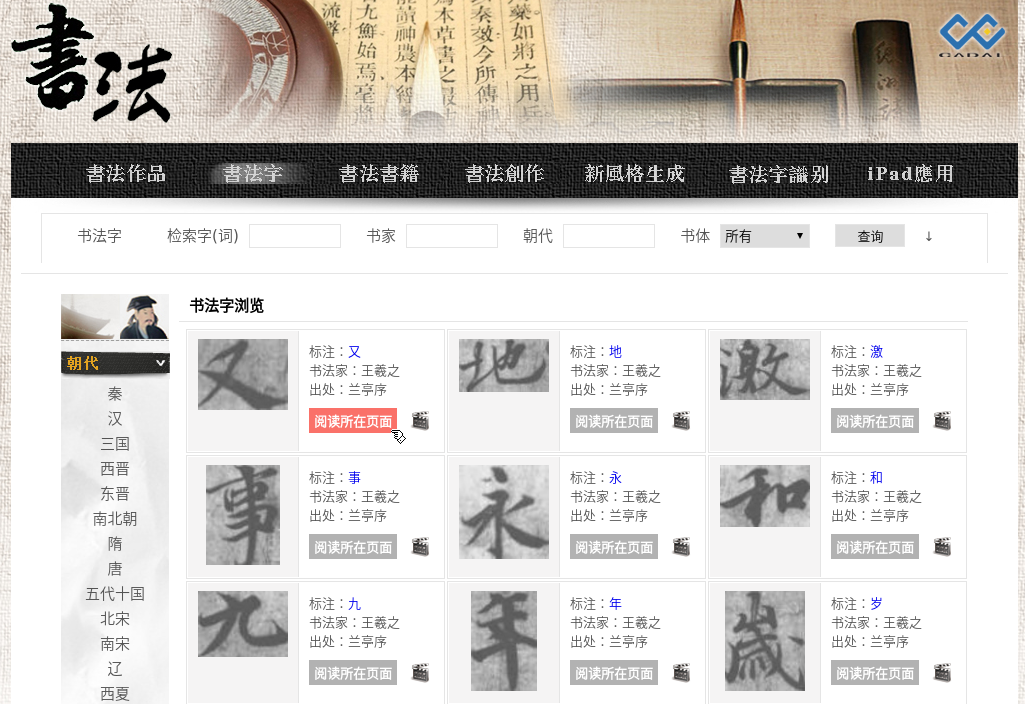
\includegraphics[width=12cm]{website-char-select.png}}
    \caption{CADAL character mode, selecting "view in page"}
    \label{Character table in CADAL}
    \end{figure}
    
    \begin{figure}[t]
    \parbox{3cm}{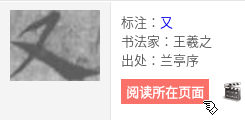
\includegraphics[width=3cm, vshift=-8cm]{website-char-select-zoomed.png}}
    \qquad
    \parbox{10cm}{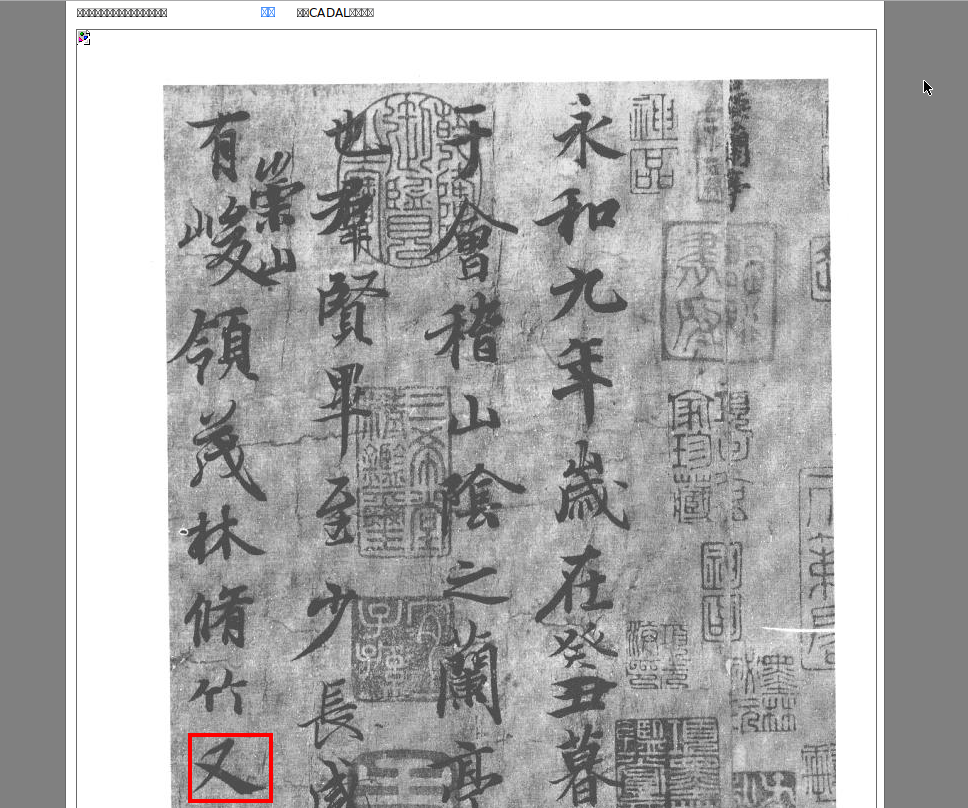
\includegraphics[width=10cm]{website-char-in-page.png}}
    \caption{selecting character brings up parent page}
    \label{selecting character brings up parent page}
    \end{figure}
    
    \begin{figure}[t]
    \parbox{12cm}{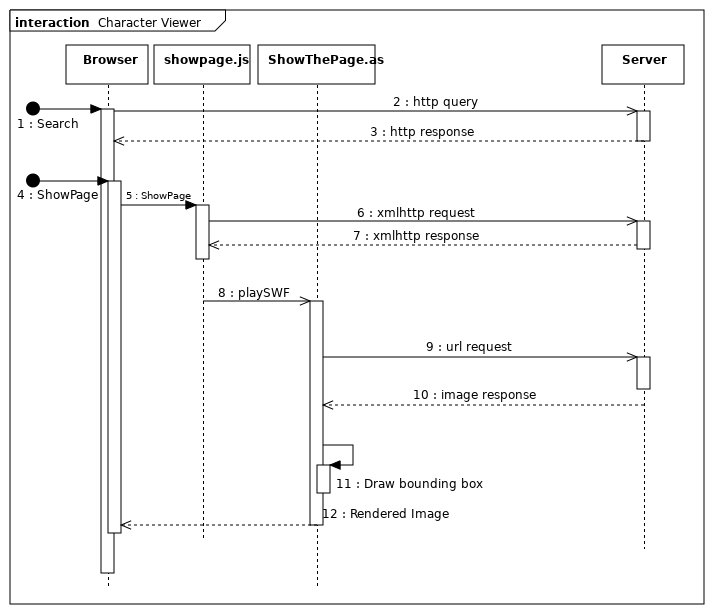
\includegraphics[width=12cm]{website-interaction-diagram.png}}
    \caption{interaction diagram: selecting "view in page"}
    \label{CADAL website interaction diagram}
    \end{figure}
    
    \begin{figure}[t]
    \parbox{12cm}{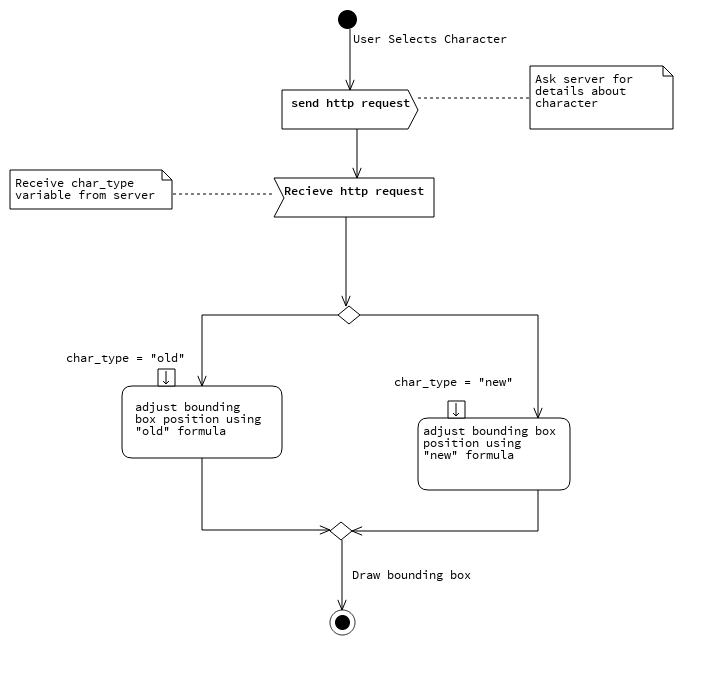
\includegraphics[width=12cm]{website-sequence-diagram.png}}
    \caption{sequence diagram: CADAL character transformation }
    \label{CADAL website sequence diagram}
    \end{figure}
    
    
    
    TODO: add explanation of the "old" and the "new formulas"
    
    (character mode)
        In this mode users may browse, search for or view individual characters.  The characters are printed in a table, with up to 18 characters visible on the page at any given time.  The following search fields are searchable:
            * character : 检索字(词)
            * calligrapher :  书家
            * dynasty :  朝代
            * Chriography :  书体 , a dropdown menu consisting of 6 different styles, all: 所有 or (楷书) (行书) (篆书) (隶书) (草书) (其它)
            
            An additional drop-down menu reveals additional search options.
            
            * 偏旁笔画 : Radical strokes, a dropdown consisting of 1, 2, 3......15 strokes
            *  偏旁 : Radical, a dropdown consisting of between 1 and 
            
            
            These additional search options all have to do with different characteristics of a single character.  example


    Both character images and page live on the CADAL server in the following structure:


.
└── CalliSources
    ├── books
    │   ├── 06100004
    │   │   └── otiff
    │   │       ├── 00000009.tiff
    │   │       ├── 00000010.tiff
    │   │       └── .....
    │   ├── 06100005
    │   └── .....
    └── images
        └── chatacterimage
            ├── 06100004
            │   ├── 00000009(266,179,402,296).jpg
            │   ├── 00000010(206,251,358,346).jpg
            │   └── .....
            ├── 06100005
            └── .....


The CADAL Server in china delivers images at wildly inconsistant speeds.  Sometimes as slow at 20KB/s sometimes as fast at 2.5MB/s.  But usally above 50KB/s and below 500KB/s.  Slow bulk data transfer is a notorious problem when transfeing information in or out of China.  It took over 5 days to retrieve about 40Gb of images and store it on my Server.

            
            
            
            The web scraping process is made up of the following steps and is generally considered more of an art than a Science.
                1)  Experiment with the website.  Discover the pattern of requests that return pages carrying the information you need.
                2)  Generate a list of requests based on step 1
                3)  Send the requests in step 2 to the website, and record the response.
                4)  Use a tool called an HTML parser to extract the required information from retrieved files.
                    *I stored the results of this step in a JSON file.
                
            I also needed to harvest the images.  Fortunately, the images lived in a part of the website that serves static content and enabled navigation throughout it's folder structure.  I found the list files / folders we needed from the web scraping performed earlier.  It became a matter of bulk HTTP requesting the images in specific folders.
            
            Importantly, I discovered higher resolution images than are displayed via the website here!  Details..... Details
            
            In total the static part of the download consisted of just over 130K images, and totaled about 40Gb of data.  This bulk download took about 2 weeks due to the very high slowdown caused by the Great Firewall of China.
            
            I then imported the results of the parsed HTML pages into a Relational Database. (PostgreSQL).  Then I linked the character and page database rows with the images bulk downloaded earlier.
            
            I performed ad-hawk verification, I ran a handful of queries from the CADAL website, and verified that the results matched the same queries in my newly generated database.   Everything matched, including the bounding box coordinates from the CADAL site.  However, the bounding boxes generated by my data were in different locations to the bounding boxes found on CADAL.
            
            
            I eventually discovered that the CADAL show page from does the following before drawing the image on the screen:
                *) The user clicks the "show" button indicating the desire to see the parent page with a box drawn abound the current character.
                *) A JavaScript app inside the site sends an Asynchronous HTTP response to the CADAL with the parent page as the payload.
                *) The script receives the response "new" or "old" from the CADAL server
                *) The script then passes the Character coordinates, as well as the above string to a SWF(Shock-Wave Flash) applet
                *) The SWF applet loads the parent page, and resizes the image to 800px wide, aspect ratio is maintained
                *) The SWF applet tests whether the string just passed in is "new", or "old"
                    *Depending on the above new/old result the SWF applet performs one of two different transformations to the coordinates
                    *Using the newly transformed coordinates the SWF applet draws a bounding box around the character.
                In order to examine the behavior of the SWF applet, I had to use a SWF decompiler, and examine the internals of the SWF applet.
            
                Based on the above information about the behavior of the bounding box drawing mechanism I performed my own set of queries to determine whether any one of my page images was "new", or "old".
                *Using this new/old information as well as the corresponding coordinate transformation embedded inside the SWF app I was able to transform the relative coordinates I fetched earlier to absolute coordinates correctly matching the pixel locations of the character in the high resolution images I'd downloaded previously.
                
                
                I now had all relevant character information, as well as corresponding work information and images to build my interface.
                
    A cursory examination of the reconstructed database revealed much of the DATA in CADAL is incomplete for the following reasons:
        * not all calligraphic works have a text script or title accompanying them
        * A large portion (Perhaps an overwhelming majority) of pages with characters lack corresponding database entries for at least some, and occasionally as much as 1/2 or more of characters in an image.
        * of those calligraphic works with characters mapped
            -pages only have a portion of characters mapped.
            -Quality of mapped characters is generally quite good except:
                Bounding boxes frequently overlap
                Bounding boxes frequently cut off portions of the character.                
    
    
    I have not acquired the following portions of the CADAL Database for my purposes:
    
    
    
    Now that I have the required information.  I can import that information into CaliSet.
